\documentclass{livrerecettes}

\usepackage{hyperref}
\hypersetup{
    colorlinks=true,
    linkcolor=blue,
    urlcolor=blue,
    citecolor=blue
}
\usepackage{anyfontsize}
\renewcommand{\normalsize}{\fontsize{11pt}{13pt}\selectfont}
\usepackage[utf8]{inputenc}
\usepackage[T1]{fontenc}
\usepackage{multicol} % requis pour la macro \ingredients
\usepackage{graphicx} % pour les images
\usepackage[french]{babel}
\usepackage{imakeidx}

% \setlength{\parskip}{1.5em} % espace entre paragraphes

\begin{document}

\title{Recettes de cuisine}
\author{Famille Poirier Ruiz Pacheco}
\date{\today}
\maketitle
% Choisir un motif d'ornement et son échelle (pgfornament ID et largeur)
% Exemple: 9, 63, 87... voir les motifs fournis par pgfornament
\renewcommand{\PageOrnamentID}{11}
\renewcommand{\PageOrnamentWidth}{1.5cm}
\renewcommand{\PageOrnamentSideXShift}{0.9cm}
\renewcommand{\PageOrnamentTopOffset}{-0.5cm} % remonté de 2.0cm par rapport à 0.2cm
% Activer les ornements de page définis par la classe
\EnablePageOrnaments

% Page avec image principale
\newpage
\thispagestyle{empty}
\vspace*{\fill}
\begin{center}
    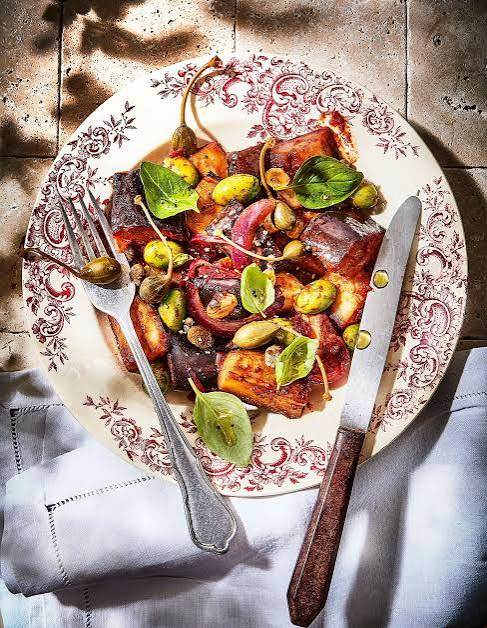
\includegraphics[width=0.8\textwidth]{images/livre}
\end{center}
\vspace*{\fill}
\newpage

\tableofcontents

\chapter{Entrées}
\newpage
\input{recettes/001_entrees/001.tex}


\chapter{Plats}
\newpage
\input{recettes/002_plats/001.tex}
\newpage
\input{recettes/002_plats/002.tex}

\chapter{Desserts}
\newpage

\input{recettes/003_desserts/001.tex}

\end{document}